So far we have considered:
\[
    \underline{y} = X\underline{w} \hspace{1cm} X \in \mathbb{R}^{n \times p} \text{ and } \begin{Bmatrix}
        \text{Least Squares}: \underline{\hat{w}}_LS\\
        \text{Ridge Regression}: \underline{\hat{w}}_{RR}\\
    \end{Bmatrix} \underline{w} \in \mathbb{R}^p \text{ dense vector, i.e. not many zeros} 
\]
We are going to see a method which obtain a vector $\underline{\hat{w}}$ with many zeros, as sparse as possible. We want to consider this model:
\[
    \underline{y} = X\underline{w} \hspace{1cm} X \in \mathbb{R}^{n \times p} \hspace{1cm} p > n 
\]
We have said that the system is undetermined since it has infinite solutions. Suppose to have 2 features and 1 sample. 
\[
    X = \begin{bmatrix}
        2 & 3\\
    \end{bmatrix}
    \hspace{1cm}
    y = \begin{bmatrix}
        1\\
    \end{bmatrix}
\]
And so:
\[
    1 = \begin{bmatrix}
        2 & 3
    \end{bmatrix}\begin{bmatrix}
        w_1\\
        w_2
    \end{bmatrix} \implies
    1 = 2w_1 + 3w_2 \hspace{0.2cm} \leftarrow \hspace{0.2cm} \text{line}    
\]
As mentioned in a previous lecture, we want to find the minimum length solution so we can plot the line found before and the circles that represents the l2-norm distance.
\begin{center}
    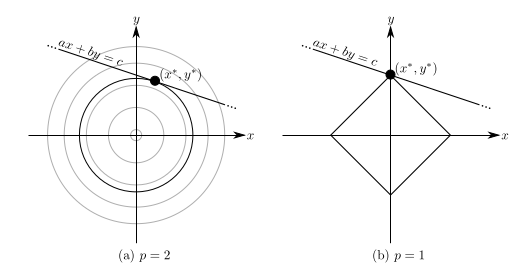
\includegraphics[scale=0.6]{../images/LassoRidgePlot.png}
\end{center}
On the right-hand side it is represented the equivalent plot but with the l1-norm. We can see that the solution on the right has one coordinate (are features!) that is equal to zero. This is true in general, i.e. we will obtain sparser solution using the l1-norm rather than the l2-norm.\\
With L1-norm it's still a convex optimization problem and
\[
    F(\underline{w}) = ||X\underline{w} - \underline{y}||_2^2 + \lambda ||\underline{w}||_1    
\] 
This model is implemented by \textbf{Lasso} (Least Absolute Shrinkage and Selection Operator) and achieve both the shortest distance solution and the selection of some features.

This is important because by reducing the number of features, we increase the interpretability of the model.\\

There is also the \textbf{Elastic Net} which combines both Lasso and Ridge: 
\[
    F(\underline{w}) = ||X\underline{w} - \underline{y}||_2^2 + \lambda_1||\underline{w}||_1 + \lambda_2||\underline{w}||_2^2  
\] 

\vspace{2cm}
Once again, we start considering:
\[
    \underline{y} \in \mathbb{R}^n \hspace{1cm} X \in \mathbb{R}^{n \times p} \hspace{0.2cm} \text{with \emph{p} lin. ind. cols } (\implies \sigma_i > 0, \hspace{0.1cm} i = 1, \dots, p)  
\]
Now we write the formulation of the weights vector $w$ we found for Ridge Regression. 
\[
    \begin{split}
    \underline{\hat{w}}_R &= V\underbrace{(\Sigma^\intercal \Sigma + \lambda I)^{-1} \Sigma^\intercal}_{\substack{\Sigma^\intercal(\Sigma \Sigma^\intercal + \lambda I)^{-1}}} U^\intercal \underline{y}\\
    &= \underbrace{V\Sigma^\intercal U^\intercal}_{X^\intercal} \underbrace{U(\Sigma \Sigma^\intercal + \lambda I)^{-1} U^\intercal \underline{y}}_{\underline{\alpha} \in \mathbb{R}^n}\\
    &= X^\intercal \underline{\alpha}\\
    &= \sum_{i=1}^n \alpha_i \underline{x}_i\\
    \end{split}     
\]
In the second passage we have added the matrices $U^\intercal U$ because its the identity matrix. We obtain a weighted sum of the column vectors of $X^\intercal$, where $X$ is:
\[
X = \begin{bmatrix}
    \horzbar & \underline{x_1^\intercal} & \horzbar\\
    \horzbar & \underline{x_2^\intercal} & \horzbar\\    
     & \vdots & \\
    \horzbar & \underline{x_n^\intercal} & \horzbar
\end{bmatrix}
\]
So, until now, we have discussed about linear models. A generic form would be:
\[
    \hat{y}_i = w_1x_{i1} + w_2x_{i2} \hspace{1cm} \text{if} \hspace{1cm} \underline{x}_i = \begin{bmatrix}
        x_{i1}\\
        x_{i2}
    \end{bmatrix}    
\]
Now a new model:
\[
    \hat{y}_i = w_1x_{i1} + w_2x_{i2} + w_3x_{i1}^2 + w_4x_{i2}^2 + w_5x_{i1}x_{i2}    
\]
So, the original feature vector $\underline{x}$ is transformed into a new feature vector by means of function called feature map $\phi(x)$:
\[
    \phi(x) = \begin{bmatrix}
        x_1\\
        x_2\\
        x_1^2\\
        x_2^2\\
        x_1x_2
    \end{bmatrix} \in \mathbb{R}^d \hspace{1cm} d > p \text{ typically}    
\]
And
\[
    \hat{y}_i = \phi(x_i)^\intercal \underline{w}    
\]
In general $d$ can be huge.


\section{Kernel Methods}
The aim of this methods is to avoid the necessity of computing huge vectors.
\[
    \Phi =  \begin{bmatrix}
        \horzbar & \phi(\underline{x}_1)^\intercal & \horzbar\\
        \horzbar & \phi(\underline{x}_2)^\intercal & \horzbar\\    
         & \vdots & \\
        \horzbar & \phi(\underline{x}_n)^\intercal & \horzbar
    \end{bmatrix}
    \in \mathbb{R}^{n \times d} \hspace{1cm} \underline{\hat{y}} = \Phi \underline{w}
\]
The objective is still the same: i.e. finding $\underline{w}$. We are now going to consider ridge regression in order to achieve that. 
Instead of $\underline{\hat{w}}_R = X^\intercal \underline{\alpha}$ we can now write:
\[
    \underline{\hat{w}}_R = \Phi^\intercal \underline{\alpha}
\]
Where
\[
    \underline{\alpha} = U(\Sigma \Sigma^\intercal + \lambda I)^{-1} U^\intercal \underline{y} = (XX^\intercal + \lambda I)^{-1} \underline{y}    
\]
Here is the proof:
\[
    (U\Sigma V^\intercal V\Sigma^\intercal U^\intercal + \lambda UU^\intercal)^{-1} \underline{y}    
\]